% Table generated by Excel2LaTeX from sheet 'Sheet1'
\begin{table}[t]
\centering
\scriptsize
\caption{Quantitative retrieval quality of different KG-based
retrieval methods.}
\resizebox{\textwidth}{!}{%
\begin{tabular}{c|cc|cc|cc}
\toprule
\multirow{2}{*}{Method} &
\multicolumn{2}{c|}{STaRK-Amazon} &
\multicolumn{2}{c|}{STaRK-MAG} &
\multicolumn{2}{c}{STaRK-PRIME} \\
\cmidrule(lr){2-7}
& $\text{Step-}\Delta_{Seper}\uparrow$ & $\text{Answer-}\Delta_{Seper}\uparrow$ & $\text{Step-}\Delta_{Seper}\uparrow$ & $\text{Answer-}\Delta_{Seper}\uparrow$ & $\text{Step-}\Delta_{Seper}\uparrow$ & $\text{Answer-}\Delta_{Seper}\uparrow$ \\
\midrule
ToG+GPT-4o & 0.031 $\pm$ 0.109 & 0.092 $\pm$ 0.128 & 0.041 $\pm$ 0.172 & 0.065 $\pm$ 0.150 & 0.065 $\pm$ 0.125 & 0.148 $\pm$ 0.165 \\
ToG+LLaMA3 & 0.010 $\pm$ 0.118 & 0.046 $\pm$ 0.149 & 0.068 $\pm$ 0.108 & 0.105 $\pm$ 0.146 & 0.009 $\pm$ 0.102 & 0.021 $\pm$ 0.106 \\
SFT & 0.079 $\pm$ 0.151 & 0.141 $\pm$ 0.160 & 0.035 $\pm$ 0.101 & 0.084 $\pm$ 0.095 & 0.062 $\pm$ 0.132 & 0.158 $\pm$ 0.183 \\
PRM & 0.029 $\pm$ 0.089 & 0.071 $\pm$ 0.112 & 0.037 $\pm$ 0.117 & 0.060 $\pm$ 0.115 & 0.057 $\pm$ 0.106 & 0.131 $\pm$ 0.174 \\
G-Retriever & --- & 0.024 $\pm$ 0.110 & --- & 0.012 $\pm$ 0.089 & --- & 0.029 $\pm$ 0.117 \\
SubgraphRAG & --- & 0.021 $\pm$ 0.093 & --- & 0.039 $\pm$ 0.076 & --- & 0.046 $\pm$ 0.083 \\
GraphFlow & \textbf{0.097 $\pm$ 0.158} & \textbf{0.219 $\pm$ 0.257} & \textbf{0.081 $\pm$ 0.137} & \textbf{0.145 $\pm$ 0.112} & \textbf{0.091 $\pm$ 0.147} & \textbf{0.206 $\pm$ 0.192} \\
\bottomrule
\end{tabular}
}
\label{tab:retrieval}
\end{table}





\subsection{Dataset}
We employ the STaRK \cite{wu2024stark} benchmark to validate the retrieval quality of the proposed GraphFlow to support complex queries.
%STaRK is a recently proposed benchmark to evaluate the retrieval performance of KG-based RAG methods consisting of text-rich KGs from three domains:
STaRK is a recently proposed benchmark designed to evaluate the retrieval performance of KG-based RAG methods on text-rich KGs spanning three domains:
\begin{itemize}
    \item \textbf{STaRK-AMAZON} is an e-commerce KG where the nodes contain detailed product information and the edges denotes the properties of products and co-purchase between products.
    The retrieval task is to retrieve the diverse products to satisfy the recommendation query.
    \item \textbf{STaRK-MAG} is an academic graph constructed based on OGB \cite{hu2020open} and Microsoft Academic Graph \cite{sinha2015overview}. The nodes contain author information, institute, and publications.
    The retrieval task is to address academic queries such as paper searching.
    \item \textbf{STaRK-PRIME} is a biomedical KG where the nodes are associated with the detailed description of drugs, disease, genes, and pathways, and the edges are their relationship.
    The retrieval task is to address the biomedical query.
\end{itemize}
The StaRK benchmark challenges KG-based RAG methods by complex queries corresponding to diverse retrieval targets and fusion of text and structure information that complicates accurate retrieval.

\subsection{Baseline and Evaluation Metrics}
\begin{figure}[t]
%\vspace{-0.3cm}
\begin{center}
%\framebox[4.0in]{$\;$}
\centerline{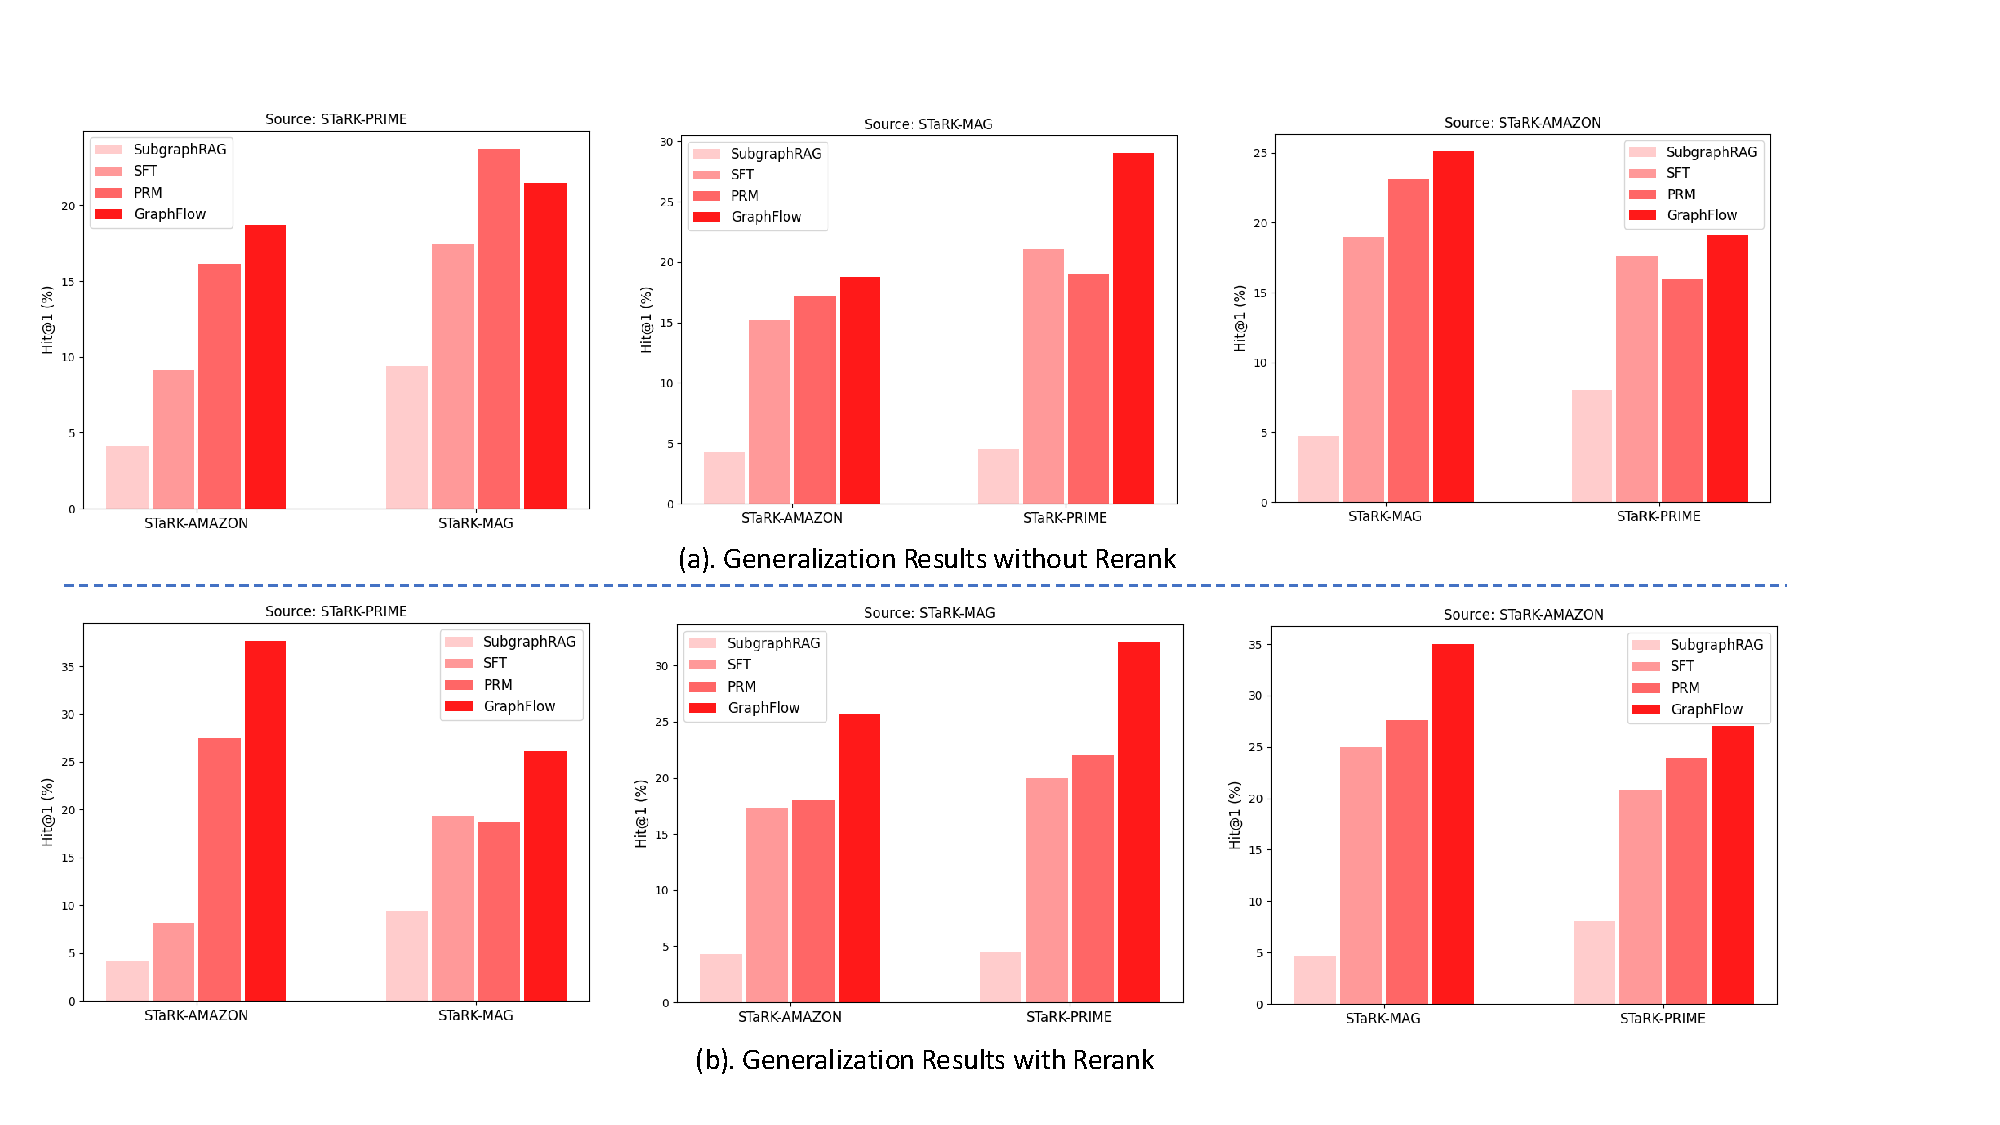
\includegraphics[width=0.9\columnwidth]{generalization.pdf}}
\end{center}
\vspace{-0.9cm}
\caption{Generalization Performance of KG-based RAG methods. GraphFlow shows superior cross-domain generalization performance, especially under the rerank setting (best viewed in color).} 
\vspace{-0.3cm}
\label{figure:generalization}
\end{figure}
\xhdr{Baseline}
We choose representative retrieval-based and agent-based baselines with explicit retrieval results (i.e., the retrieved node index) on the STaRK benchmark \cite{wu2024stark}. All detailed implementations are shown in Supplementary Material due to space limit.

For retrieval-based baselines, we consider \textbf{Dense-Retriever} \cite{karpukhin2020dense}, \textbf{G-Retriever} \cite{he2024g}, and \textbf{SubgraphRAG} \cite{liretrieval}.
Dense-Retriever is implemented with SentenceBERT \cite{reimers2019sentence} to encode both questions and the documents of KG nodes into dense embeddings and retrieve the documents with top vector similarity.
G-Retriever employs the Prize-Collecting Steiner Tree (PCST) \cite{archer2011improved} algorithm to extract a subgraph from KGs relevant to the query. 
Since computing PCST on STaRK benchmark is infeasible, we follow the hybrid setting \cite{lee2024hybgrag,lei2025mixture} that first identifies a source node in KG via Dense-Retriever and only computes PCST around the ego-graph up to 2 hops around the identified node.
We also adopt the same hybrid setting for other baselines to ensure computational feasibility on STaRK.
SubgraphRAG integrates a learnable subgraph retrieval module to retrieve from KG.

For agent-based methods, we consider \textbf{ToG} \cite{sunthink}, \textbf{SFT}, and \textbf{PRM} \cite{lightman2023let} as baselines.
ToG employs an LLM agent to search from the KG to retrieve supporting documents. 
We instantiate ToG using both LLaMA3-8B-Instruct and GPT-4o as backbone models, denoted as ToG+LLaMA3 and ToG+GPT4o, respectively.
SFT and PRM are two popular approaches that fine-tune the LLM agent to enhance RAG in recent works \cite{xiong2025rag,dong2025understand,huang2025rag}. SFT, PRM, and GraphFlow are deployed with LLaMA3-8B-Instruct \cite{grattafiori2024llama}.
For agent-based methods, we use the agent to rerank all the retrieved results.

\xhdr{Evaluation Metrics}
All KG-based RAG methods retrieve every input query 20 times and generate 20 retrieval results for diversity and accuracy evaluation following the standard setting in STaRK \cite{wu2024stark}. 
We employ the following metrics to evaluate the retrieval performance. Hit@k denotes whether the ground truth is retrieved in the top-k results. We employ \textbf{Hit@1 and Hit@5} to measure the retrieval precision of the different KG-based RAG methods. \textbf{Mean Reciprocal Rank (MRR)} measures the average of reciprocal ranks of the first ground-truth item in the retrieval results and encourages the ground-truth item to be retrieved in a higher rank. \textbf{Recall@k (R@k)} is a standard metric to measure the percentage of ground-truth items that appear in the top-$k$ retrieved results. We employ Recall@20 (R@20) for evaluation. \textbf{De-duplicate Recall@k (D-R@k)} measures the percentage of \textit{unique} ground-truth items that appear in the top-$k$ retrieved results. This metric is used to evaluate the diversity of the correctly retrieved results. We use De-duplicate Recall@20 (D-R@20).
% \begin{itemize}
%     \item \textbf{Hit@k} denotes whether the ground truth is retrieved in the top-k results. We employ Hit@1 and Hit@5 to measure the retrieval precision of the different KG-based RAG methods.
%     \item \textbf{Mean Reciprocal Rank (MRR)} measures the average of reciprocal ranks of the first ground-truth item in the retrieval results and encourages the ground truth item to be retrieved in a higher rank.
%     \item \textbf{Recall@k (R@k)} is a standard metric to measure the percentage of ground-truth items that appear in the top-$k$ retrieved results. We employ Recall@20 (R@20) for evaluation.
%     \item \textbf{De-duplicate Recall@k (D-R@k)} measures the percentage of \textit{unique} ground-truth items that appear in the top-$k$ retrieved results. This metric is used to evaluate the diversity of the correct retrieved results. We employ De-duplicate Recall@20 (D-R@20) for evaluation.
% \end{itemize}
\subsection{Main Results}
\xhdr{Accuracy}
Table~\ref{tab:performance-retrieval-acc} presents the retrieval accuracy of various KG-based RAG methods on STaRK.
\begin{wrapfigure}{r}{6.0cm}
\vspace{-0.3cm}
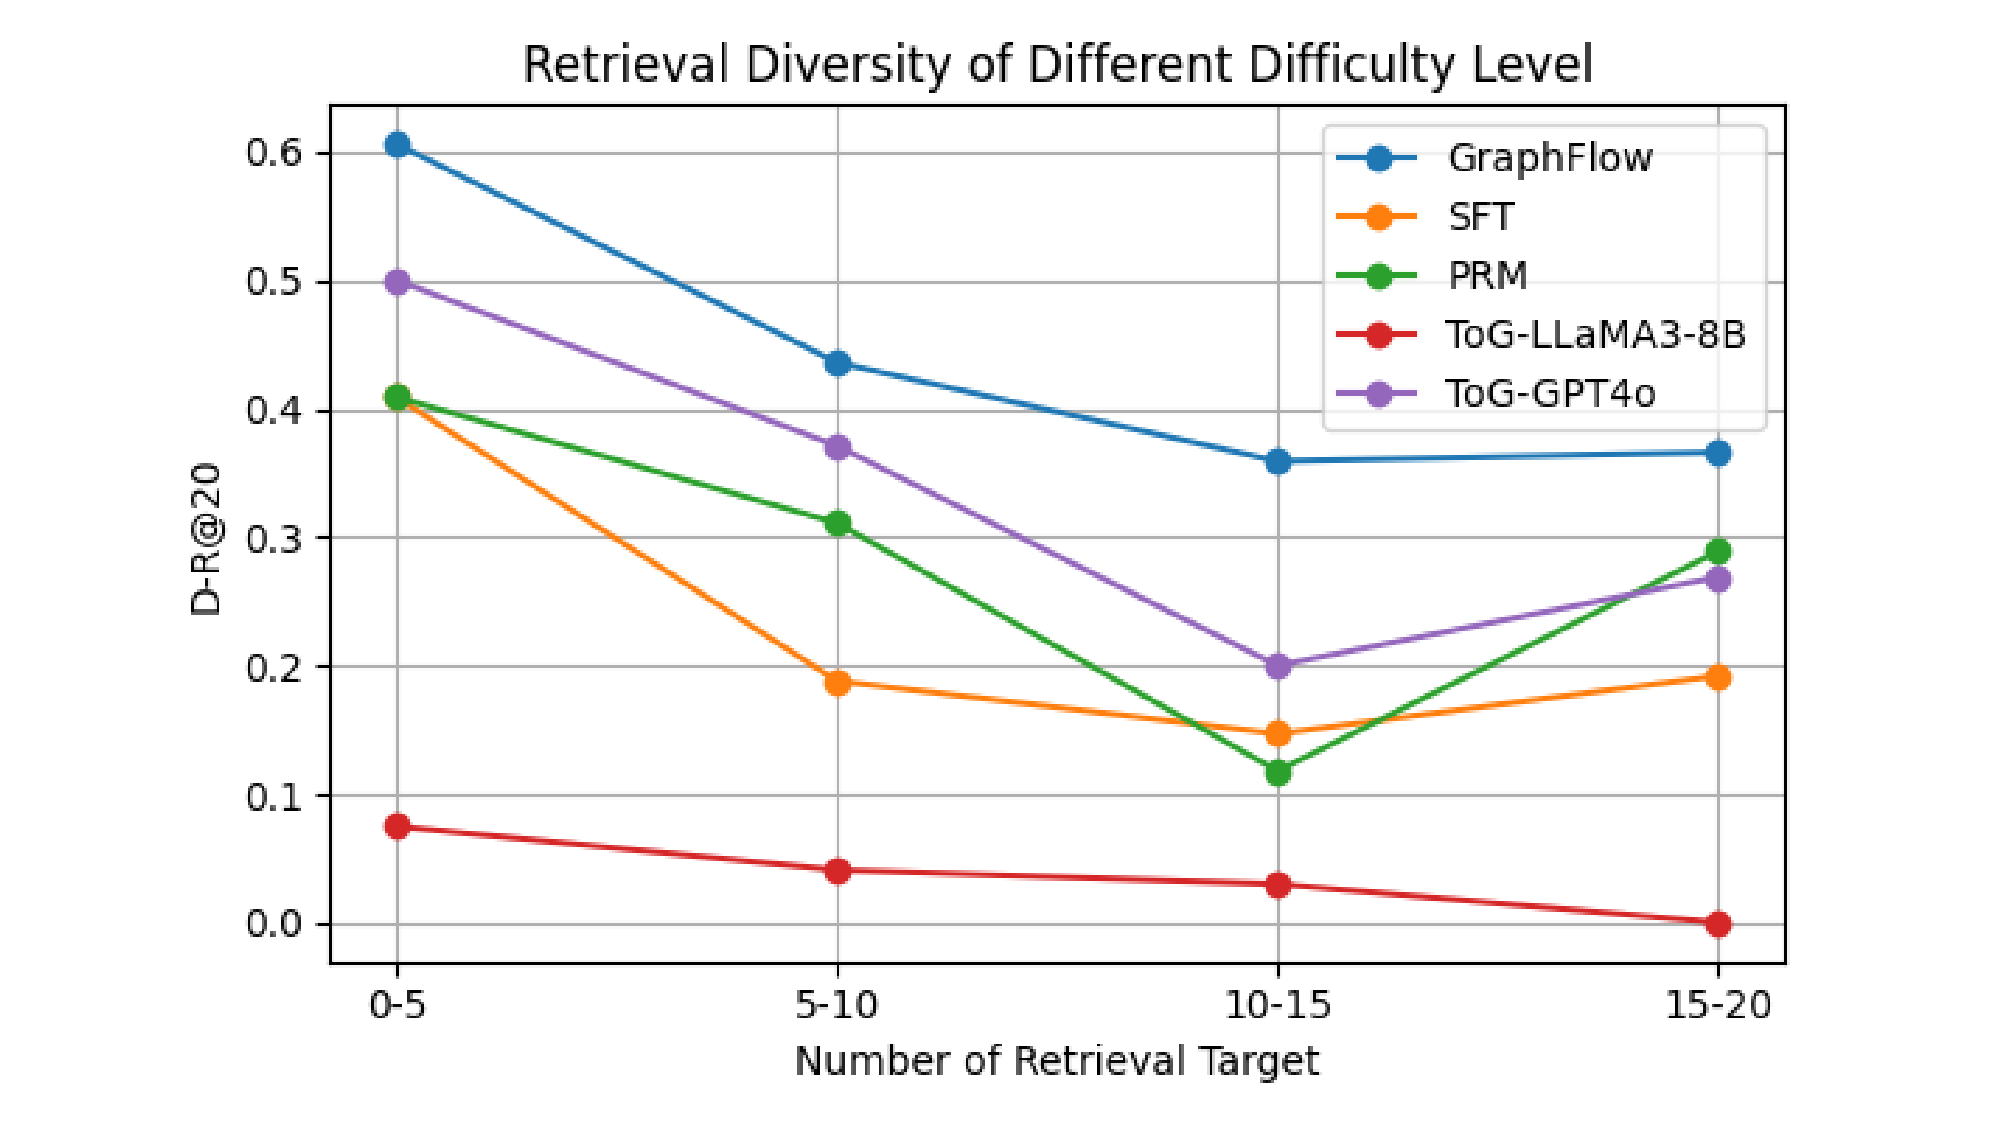
\includegraphics[width=1.0\linewidth]{hard_case.pdf}
\vspace{-0.6cm}
\caption{GraphFlow shows improved retrieval diversity on different difficulty levels of retrieval queries on STaRK-PRIME.} 
\vspace{-0.2cm}
\label{figure:hard_case}
\end{wrapfigure}
GraphFlow consistently outperforms other KG-based RAG approaches on most metrics.
In particular, it achieves higher Hit rates and MRR scores than the strong baseline ToG+GPT-4o with an average 10\% improvement in retrieval accuracy.
Interestingly, ToG’s performance is highly sensitive to the choice of backend model.
When instantiated with LLaMA3-8B, ToG shows a significant drop in performance compared to using GPT-4o.
Additionally, rerank has no effect in the ToG+LLaMA3-8B setup, as all retrieved results receive equally high scores, leaving the ranking unchanged.

Two finetuned agent-based baselines, SFT and PRM, outperform ToG without finetuning, but still fall short of GraphFlow.
While PRM training can leverage curated preference datasets with fine-grained process-level rewards, such labeling is prohibitively expensive.
Instead, GraphFlow achieves high-quality retrieval with only outcome rewards of retrieval trajectories.
For retriever-based approaches, DenseRetriever, G-Retriever, and SubgraphRAG show moderate performance but are generally inferior to agent-based methods.
Overall, retriever-based methods remain more lightweight but trail behind agent-based approaches in retrieval accuracy.


\xhdr{Diversity}
Table~\ref{tab:performance-retrieval-diversity} reports the retrieval diversity of different KG-based RAG methods on the STaRK benchmark.
We evaluate both Recall@20 (R@20) and its de-duplicated variant (D-R@20), which better captures retrieval diversity.
GraphFlow achieves the highest retrieval diversity across all datasets, outperforming both retriever-based and agent-based baselines.
Its results not only match more ground-truth contents but also avoid redundancy.
Notably, GraphFlow exceeds the strongest baseline (ToG+GPT-4o) by a large margin on the STaRK-PRIME dataset, highlighting its ability to retrieve results that are both relevant and diverse.
Compared with PRM and SFT, GraphFlow also demonstrates superior diversity.
In contrast, retriever-based methods retrieve less diverse content and cover fewer retrieval targets.

% \xhdr{Accuracy} The retrieval accuracy of various KG-based methods on three datasets is shown in Table~\ref{tab:performance-retrieval-acc}. 
% GraphFlow outperforms the other KG-based RAG methods and achieves the highest retrieval accuracy across three datasets.
% Especially, GraphFlow achieves higher Hit rates and MRR scores on most datasets than strong agent-based approaches and leads to an average 10\% performance gain over ToG+GPT4o.
% Notably, the performance of ToG is sensitive to its backend model. When employ LLaMA3-8B to instantiate ToG, we observe a significant performance decline compared with initiation ToG with GPT-4o.
% We also observe that rerank does not change the performance of ToG+LLaMA3-8B since the all the retrieved results are assigned with the highest scores and reranking does not change the order in the retrieved results.
% SFT and PRM are two baselines that finetunes LLM agent for KG-based RAG. 
% These methods outperform ToG that do not fine-tune LLM. However, they still underperform GraphFlow since high-quality process-level supervision is still expensive.
% Among retriever-based approaches, DenseRetriever and PCST exhibit moderate performance but fall short compared to agent-based methods, highlighting the limitations of non-parametric retrieval in complex reasoning tasks. 
% SubgraphRAG employs a parameterized small MLP as the retriever model and outperforms DenseRetriever and PCST.
% Overall, the retrieval accuracy of retriever-based approaches lags behind agent-based approaches, but retriever-based approaches also offer a light-weight solution under low source settings.

% \xhdr{Diversity} 
% Table~\ref{tab:performance-retrieval-diversity} demonstrates the retrieval diversity of different KG-based RAG methods across the Amazon, MAG, and PRIME datasets. We report both Recall@20 (R@20) and its de-duplicate variant (D-R@20), which better measures diversity.
% GraphFlow achieves higher diversity in correct retrieval results across all datasets than both retriever-based and agent-based baselines. 
% Moverover, the retrieval results of GraphFlow cover more ground-truth contents for the queries than other baselines.
% Notably, GraphFlow significantly surpasses the best baseline (ToG+GPT4) by a large margin on PIRME, 
% indicating its strong capability to retrieve not only accurate but also diverse results to support the query. 
% Compared with PRM and SFT that also fine-tune the LLM, GraphFlow also demonstrates higher retrieval diversity, showing its effectiveness in avoiding redundant retrieval results.
% In contrast, retriever-based methods struggle with less diverse retrieval results and cover less ground-truth content.
\subsection{Quantifying Retrieval Quality}
We further employ the Seper score ($\Delta_{Seper}$) \cite{daiseper} to quantify the retrieval quality of different KG-based retrieval methods.
The Seper score is a recently proposed metric for evaluating retrieval utility by measuring semantic perplexity reduction after retrieval: $\Delta_{Seper}=p_{M}(a|q,d)-p_{M}(a|q)$. 
Here, $q$ is the question, $d$ is the document associated with the retrieval item, and $M$ is an LLM used for question answering. In our case, we use LLaMA3–8B–Instruct to instantiate $M$ to keep consistent with the retrieval model.
Since there is no ground-truth answer for the questions in the STaRK benchmark, we use the title or summarized description of the ground-truth retrieval item as $a$. 
We design the following metrics for comprehensive evaluation and report their mean and standard deviation (std).
\begin{itemize}
    \item $\text{Step-}\Delta_{Seper}$: the Seper score that quantity the retrieval quality of intermediate retrieval.
    \item $\text{Answer-}\Delta_{Seper}$: the Seper score that quantity the retrieval quality of the final result.
\end{itemize}
As shown in Table~\ref{tab:retrieval}, GraphFlow consistently achieves higher $\text{Step-}\Delta_{Seper}$ and $\text{Answer-}\Delta_{Seper}$ than all the baselines, demonstrating stronger information utility during retrieval. 
These results further confirm that GraphFlow can significantly improve the information utility when retrieving from text-rich KGs.
Notice that all the methods have high variance in $\text{Step-}\Delta_{Seper}$ and $\text{Answer-}\Delta_{Seper}$.
The reason is the high variance in natural language entailment when calculating Seper scores.
Moreover, we observe that some retrieval samples have negative Seper scores for all methods, indicating a negative impact on question answering when retrieving bad contents.

\subsection{Further Discussion}

\xhdr{Cross-domain Generalization} Figure~\ref{figure:generalization} reports the cross-domain generalization ability of different KG-based RAG methods.
We use Hit@1 to evaluate the retrieval accuracy
Compared with SubgraphRAG using a small model for retrieval,
SFT, PRM, and GraphFlow that finetune the LLM show better cross-domain generalization ability due to the \textit{over-parameterization} \cite{leike2018scalable,gao2023scaling}. 
%Moreover, GraphFlow shows the best cross-generalization performance as it does not adopt the likelihood maximization objective as SFT or PRM.
GraphFlow demonstrates superior cross-domain generalization, since it avoids from likelihood maximization objectives used by SFT and PRM.
Instead, GraphFlow adaptively assigns the outcome reward of the retrieval trajectory to the flow values of intermediate states and guides the retrieval policy, leading to better generalization ability.
More results are shown in Supplementary Material due to space limit.

\xhdr{Performance on Hard Cases} 
We categorize the retrieval queries with different numbers of retrieval targets into 4 difficulty levels.
Figure~\ref{figure:hard_case} shows the D-R@20 scores of KG-based RAG methods on retrieval queries on STaRK-PRIME at different levels.
GraphFlow outperforms the other agent-based approaches by a large margin by covering more diverse and accurate retrieval targets, especially on the hard cases containing more than 15 retrieval targets.
The performance on hard cases shows the superior performance of GraphFlow in retrieving more relevant and diverse results.
More results of hard cases are shown in Supplementary Materials due to space limit.









